% Figure from MATH 591 notes, section 44. Compile with the notes preamble.
\begin{tikzpicture}[scale=0.9]
\draw[->, gray!50] (-2.00,0) -- (2.00,0) node[right, font=\scriptsize, text=gray!70!black] {$x$};
\draw[->, gray!50] (0.00,-2.0) -- (0.00,2.0) node[above, font=\scriptsize, text=gray!70!black] {$y$};
\draw[gray!30, dashed] (0.00,0) circle (0.60);
\draw[gray!30, dashed] (0.00,0) circle (1.10);
\draw[gray!30, dashed] (0.00,0) circle (1.60);
\draw[->, violet!75!black, thick] (-1.657,-1.343) -- (-1.343,-1.657);
\draw[->, violet!75!black, thick] (-1.605,-0.843) -- (-1.395,-1.157);
\draw[->, violet!75!black, thick] (-1.552,-0.343) -- (-1.448,-0.657);
\draw[->, violet!75!black, thick] (-1.500,0.158) -- (-1.500,-0.158);
\draw[->, violet!75!black, thick] (-1.448,0.657) -- (-1.552,0.343);
\draw[->, violet!75!black, thick] (-1.395,1.157) -- (-1.605,0.843);
\draw[->, violet!75!black, thick] (-1.343,1.657) -- (-1.657,1.343);
\draw[->, violet!75!black, thick] (-1.157,-1.395) -- (-0.843,-1.605);
\draw[->, violet!75!black, thick] (-1.105,-0.895) -- (-0.895,-1.105);
\draw[->, violet!75!black, thick] (-1.052,-0.395) -- (-0.948,-0.605);
\draw[->, violet!75!black, thick] (-1.000,0.105) -- (-1.000,-0.105);
\draw[->, violet!75!black, thick] (-0.948,0.605) -- (-1.052,0.395);
\draw[->, violet!75!black, thick] (-0.895,1.105) -- (-1.105,0.895);
\draw[->, violet!75!black, thick] (-0.843,1.605) -- (-1.157,1.395);
\draw[->, violet!75!black, thick] (-0.657,-1.448) -- (-0.343,-1.552);
\draw[->, violet!75!black, thick] (-0.605,-0.948) -- (-0.395,-1.052);
\draw[->, violet!75!black, thick] (-0.552,-0.448) -- (-0.448,-0.552);
\draw[->, violet!75!black, thick] (-0.500,0.052) -- (-0.500,-0.052);
\draw[->, violet!75!black, thick] (-0.448,0.552) -- (-0.552,0.448);
\draw[->, violet!75!black, thick] (-0.395,1.052) -- (-0.605,0.948);
\draw[->, violet!75!black, thick] (-0.343,1.552) -- (-0.657,1.448);
\draw[->, violet!75!black, thick] (-0.158,-1.500) -- (0.158,-1.500);
\draw[->, violet!75!black, thick] (-0.105,-1.000) -- (0.105,-1.000);
\draw[->, violet!75!black, thick] (-0.052,-0.500) -- (0.052,-0.500);
\draw[->, violet!75!black, thick] (0.052,0.500) -- (-0.052,0.500);
\draw[->, violet!75!black, thick] (0.105,1.000) -- (-0.105,1.000);
\draw[->, violet!75!black, thick] (0.158,1.500) -- (-0.158,1.500);
\draw[->, violet!75!black, thick] (0.343,-1.552) -- (0.657,-1.448);
\draw[->, violet!75!black, thick] (0.395,-1.052) -- (0.605,-0.948);
\draw[->, violet!75!black, thick] (0.448,-0.552) -- (0.552,-0.448);
\draw[->, violet!75!black, thick] (0.500,-0.052) -- (0.500,0.052);
\draw[->, violet!75!black, thick] (0.552,0.448) -- (0.448,0.552);
\draw[->, violet!75!black, thick] (0.605,0.948) -- (0.395,1.052);
\draw[->, violet!75!black, thick] (0.657,1.448) -- (0.343,1.552);
\draw[->, violet!75!black, thick] (0.843,-1.605) -- (1.157,-1.395);
\draw[->, violet!75!black, thick] (0.895,-1.105) -- (1.105,-0.895);
\draw[->, violet!75!black, thick] (0.948,-0.605) -- (1.052,-0.395);
\draw[->, violet!75!black, thick] (1.000,-0.105) -- (1.000,0.105);
\draw[->, violet!75!black, thick] (1.052,0.395) -- (0.948,0.605);
\draw[->, violet!75!black, thick] (1.105,0.895) -- (0.895,1.105);
\draw[->, violet!75!black, thick] (1.157,1.395) -- (0.843,1.605);
\draw[->, violet!75!black, thick] (1.343,-1.657) -- (1.657,-1.343);
\draw[->, violet!75!black, thick] (1.395,-1.157) -- (1.605,-0.843);
\draw[->, violet!75!black, thick] (1.448,-0.657) -- (1.552,-0.343);
\draw[->, violet!75!black, thick] (1.500,-0.158) -- (1.500,0.158);
\draw[->, violet!75!black, thick] (1.552,0.343) -- (1.448,0.657);
\draw[->, violet!75!black, thick] (1.605,0.843) -- (1.395,1.157);
\draw[->, violet!75!black, thick] (1.657,1.343) -- (1.343,1.657);
\draw[->, gray!50] (3.40,0) -- (7.40,0) node[right, font=\scriptsize, text=gray!70!black] {$x$};
\draw[->, gray!50] (5.40,-2.0) -- (5.40,2.0) node[above, font=\scriptsize, text=gray!70!black] {$y$};
\draw[teal!45, dashed] (5.40,0) circle (0.60);
\draw[teal!45, dashed] (5.40,0) circle (1.10);
\draw[teal!45, dashed] (5.40,0) circle (1.60);
\draw[->, teal!65!black, thick] (4.058,-1.343) -- (3.743,-1.657);
\draw[->, teal!65!black, thick] (4.058,-0.895) -- (3.743,-1.105);
\draw[->, teal!65!black, thick] (4.058,-0.448) -- (3.743,-0.552);
\draw[->, teal!65!black, thick] (4.058,0.000) -- (3.743,0.000);
\draw[->, teal!65!black, thick] (4.058,0.448) -- (3.743,0.552);
\draw[->, teal!65!black, thick] (4.058,0.895) -- (3.743,1.105);
\draw[->, teal!65!black, thick] (4.058,1.343) -- (3.743,1.657);
\draw[->, teal!65!black, thick] (4.505,-1.343) -- (4.295,-1.657);
\draw[->, teal!65!black, thick] (4.505,-0.895) -- (4.295,-1.105);
\draw[->, teal!65!black, thick] (4.505,-0.448) -- (4.295,-0.552);
\draw[->, teal!65!black, thick] (4.505,0.000) -- (4.295,0.000);
\draw[->, teal!65!black, thick] (4.505,0.448) -- (4.295,0.552);
\draw[->, teal!65!black, thick] (4.505,0.895) -- (4.295,1.105);
\draw[->, teal!65!black, thick] (4.505,1.343) -- (4.295,1.657);
\draw[->, teal!65!black, thick] (4.953,-1.343) -- (4.848,-1.657);
\draw[->, teal!65!black, thick] (4.953,-0.895) -- (4.848,-1.105);
\draw[->, teal!65!black, thick] (4.953,-0.448) -- (4.848,-0.552);
\draw[->, teal!65!black, thick] (4.953,0.000) -- (4.848,0.000);
\draw[->, teal!65!black, thick] (4.953,0.448) -- (4.848,0.552);
\draw[->, teal!65!black, thick] (4.953,0.895) -- (4.848,1.105);
\draw[->, teal!65!black, thick] (4.953,1.343) -- (4.848,1.657);
\draw[->, teal!65!black, thick] (5.400,-1.343) -- (5.400,-1.657);
\draw[->, teal!65!black, thick] (5.400,-0.895) -- (5.400,-1.105);
\draw[->, teal!65!black, thick] (5.400,-0.448) -- (5.400,-0.552);
\draw[->, teal!65!black, thick] (5.400,0.448) -- (5.400,0.552);
\draw[->, teal!65!black, thick] (5.400,0.895) -- (5.400,1.105);
\draw[->, teal!65!black, thick] (5.400,1.343) -- (5.400,1.657);
\draw[->, teal!65!black, thick] (5.848,-1.343) -- (5.953,-1.657);
\draw[->, teal!65!black, thick] (5.848,-0.895) -- (5.953,-1.105);
\draw[->, teal!65!black, thick] (5.848,-0.448) -- (5.953,-0.552);
\draw[->, teal!65!black, thick] (5.848,0.000) -- (5.953,0.000);
\draw[->, teal!65!black, thick] (5.848,0.448) -- (5.953,0.552);
\draw[->, teal!65!black, thick] (5.848,0.895) -- (5.953,1.105);
\draw[->, teal!65!black, thick] (5.848,1.343) -- (5.953,1.657);
\draw[->, teal!65!black, thick] (6.295,-1.343) -- (6.505,-1.657);
\draw[->, teal!65!black, thick] (6.295,-0.895) -- (6.505,-1.105);
\draw[->, teal!65!black, thick] (6.295,-0.448) -- (6.505,-0.552);
\draw[->, teal!65!black, thick] (6.295,0.000) -- (6.505,0.000);
\draw[->, teal!65!black, thick] (6.295,0.448) -- (6.505,0.552);
\draw[->, teal!65!black, thick] (6.295,0.895) -- (6.505,1.105);
\draw[->, teal!65!black, thick] (6.295,1.343) -- (6.505,1.657);
\draw[->, teal!65!black, thick] (6.743,-1.343) -- (7.058,-1.657);
\draw[->, teal!65!black, thick] (6.743,-0.895) -- (7.058,-1.105);
\draw[->, teal!65!black, thick] (6.743,-0.448) -- (7.058,-0.552);
\draw[->, teal!65!black, thick] (6.743,0.000) -- (7.058,0.000);
\draw[->, teal!65!black, thick] (6.743,0.448) -- (7.058,0.552);
\draw[->, teal!65!black, thick] (6.743,0.895) -- (7.058,1.105);
\draw[->, teal!65!black, thick] (6.743,1.343) -- (7.058,1.657);
\node[font=\footnotesize, violet!75!black] at (0,2.75) {$\theta = \tfrac12(x\,dy - y\,dx)$};
\node[font=\footnotesize, teal!65!black] at (5.4,2.75) {$\sigma = \tfrac12(x\,dx + y\,dy) = d\big(\tfrac14(x^2+y^2)\big)$};
\node[font=\scriptsize, align=center] at (0,-2.45) {arrows run along the circles:\\ not the gradient of any $f$};
\node[font=\scriptsize, align=center] at (5.4,-2.45) {arrows cross the level circles of $f$\\ at right angles: a gradient};
\end{tikzpicture}
